\ifx\wholebook\relax \else

\documentclass{ctexart}
\usepackage[nomarginpar
  %, margin=.5in
]{geometry}

\addtolength{\oddsidemargin}{-0.05in}
\addtolength{\evensidemargin}{-0.05in}
\addtolength{\textwidth}{0.1in}
\usepackage[cn]{../../../prelude}

\setcounter{page}{1}

\begin{document}

\title{B树}

\author{刘新宇
\thanks{{\bfseries 刘新宇 } \newline
  Email: liuxinyu95@gmail.com \newline}
  }

\maketitle
\fi

\markboth{B树}{基本算法}

\ifx\wholebook\relax
\chapter{B树}
\numberwithin{Exercise}{chapter}
\fi

\section{简介}
\index{B树}
\label{introduction}

上一章介绍的整数前缀树利用二叉树的边来表达信息。另一种扩展二叉树的方法是将分枝的数目从2增加到$k$。B树是一种自平衡的$k$叉搜索树\cite{wiki-b-tree}。它被广泛用于计算机文件系统(基于B+树,一种B树的扩展形势)和数据库系统。图\ref{fig:btree-example}展示了一棵B树,我们可以观察它和二叉搜索树之间的异同。

\begin{figure}[htbp]
  \centering
  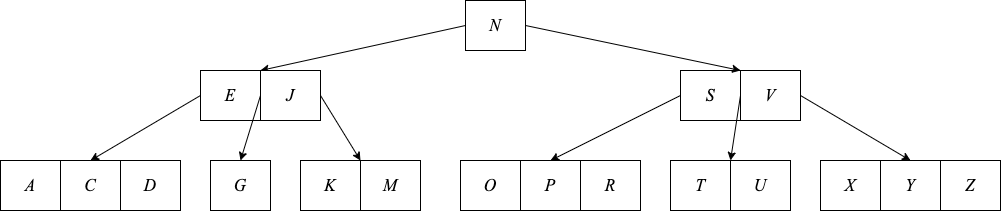
\includegraphics[scale=0.33]{img/btree-del-before.png}
  \caption{B树}
  \label{fig:btree-example}
\end{figure}

一棵二叉搜索树或者为空,或者包含一个元素$k$和左右分枝$l$、$r$。左子树$l$中的任何元素都小于$k$,并且$k$小于右子树$r$中的任何元素\footnote{严格来说,节点中可以保存键(key)和对应的值(value)。值不是必需的。简单起见,本章忽略了节点中的值,称树中保存的内容为“元素”。}:

对于非空的二叉树$(L, k, R)$,其中$L$、$R$和$k$分别代表左右子树和元素。若函数$Key(T)$可以获取树$T$的元素,这一限制条件可以表示为如下形式:

\be
\forall\ x \in l, y \in r \Rightarrow x < k < y
\ee

B树将这一思想推广到多个元素和分枝。一棵B树或者为空,括者包含$n$个元素和$n + 1$个子分枝,每个分枝也都是一棵B树。记这些元素为$k_1, k_2, ..., k_n$,分枝为$t_1, t_2, ..., t_n, t_{n+1}$,如图\ref{fig:btree-node}所示:

\begin{figure}[htbp]
  \centering
  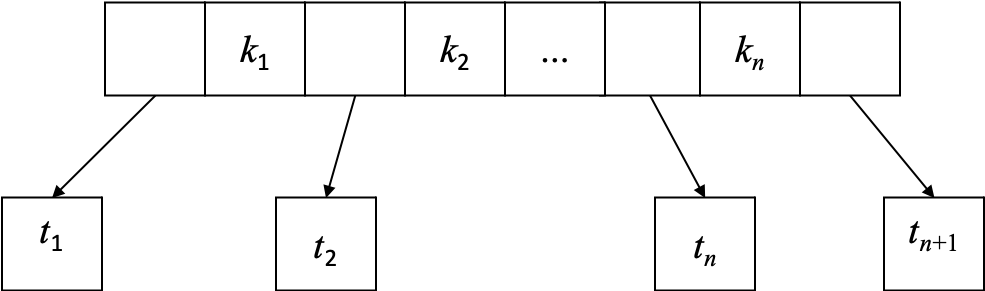
\includegraphics[scale=0.5]{img/btree-node.png}
  \caption{B树节点}
  \label{fig:btree-node}
\end{figure}

节点中的元素和分枝满足以下条件:

\begin{itemize}
\item 元素是递增的:$k_1 \leq k_2 \leq ... \leq k_n$;
\item 对于任意$k_i$,子树$t_i$中的所有元素都小于$k_i$,并且$k_i$小于子树$t_{i+1}$的任意元素。
\end{itemize}

\begin{equation}
\forall\ x_i \in t_i, i=0, 1, ..., n\ \Rightarrow x_1 < k_1 < x_2 < k_2 < ... < x_n < k_n < x_{n+1}
\label{eq:btree-order}
\end{equation}

叶子节点不包含子分枝。令元素的类型为$K$,则B树的类型为$BTree\ K$或\texttt{BTree<K>}。此外,我们还需定义一组规则以保持B树平衡:

\begin{itemize}
\item 所有的叶子节点都有相同的深度;
\item 定义整数$d$,称为B树的\underline{最小度数},每个节点:
    \begin{itemize}
        \item 最多含有$2d - 1$个元素;
        \item 最少含有$d - 1$个元素,根节点例外。
    \end{itemize}
\end{itemize}

即:

\be
  d - 1 \leq |keys(t)|  \leq 2d - 1
\ee

我们接下来证明这些规则使得B树是平衡的。

\begin{proof}
考虑一棵含有$n$个元素的B树,最小度数$d \geq 2$,树的高度为$h$。除根节点外,其它节点至少含有$d - 1$个元素。根节点至少含有一个元素。如果它有子分枝,则至少有两个深度为1的子分枝,至少有$2d$个深度为2的子分枝,至少有$2d^2$个深度为3的子分枝……最后,至少有$2d^{h-1}$个深度为$h$的叶子节点。除根节点外,将节点个数乘以$d - 1$,B树中存储的元素个数满足下面的不等式:

\be
\begin{array}{rl}
n & \geq 1 + (d - 1)(2 + 2d + 2d^2 + ... + 2d^{h-1}) \\
  & = 1 + 2(d - 1) \displaystyle \sum_{k=0}^{h-1} d^k \\
  & = 1 + 2(d - 1) \displaystyle \frac{d^h-1}{d-1} \\
  & = 2d^h - 1
\end{array}
\ee

因此树的高度满足对数关系不等式:

\be
h \leq \log_d \frac{n+1}{2}
\ee

\end{proof}

这就证明了B树的平衡性。最简单的B树称为2-3-4树。它的最小度数$t=2$,除根节点外的任何节点都包含2到4个键值。任何一棵红黑树本质上都可以转换为一棵2-3-4树。

下面的Python例子代码给出了B树的定义。它根据传入的最小度数$t$创建一个节点:

\lstset{language=Python}
\begin{lstlisting}
class BTree:
    def __init__(self, t):
        self.t = t
        self.keys = []
        self.children = []
\end{lstlisting}

B树的节点通常还保存有额外的数据(卫星数据),为了简化问题,我们暂时不考虑这些额外数据。

本章中,我们首先介绍如何通过插入操作构造B树。为了保持平衡,我们会介绍一种方法\cite{CLRS},将过满的节点在插入前进行拆分;此外,我们会介绍另外一种和红黑树类似的方法,它采用先插入后调整的策略\cite{okasaki} \cite{wiki-b-tree}。最后,我们会介绍B树的删除和查找算法。


% ================================================================
%                 Insertion
% ================================================================
\section{插入}
\index{B树!插入}
\label{btree-insertion}

我们可以通过不断插入key来构建B树。方法和二叉搜索树类似。当插入$x$时,从根节点开始,我们在节点中找到一个位置,这个位置左侧的所有key都小于$x$,而右侧的所有key都大于$x$\footnote{实际上,元素只需支持小于比较和等于比较。参见本章练习题。}。如果当前节点是叶子节点,并且没有满(节点中含有的key不足$2t-1$个),就可以将$x$插入到这个位置。否则,这一位置会指向一个子节点,我们需要递归向这一子节点插入$x$。

\begin{figure}[htbp]
  \centering
  \subcaptionbox{将22插入2-3-4树:$22 > 20$,插入右子树;$22 < 26$,插入第一个子节点。}{\includegraphics[scale=0.5]{img/btree-insert-simple1.ps}} \\
  \subcaptionbox{$21 < 22 < 25$,且叶子节点未满。}{\includegraphics[scale=0.5]{img/btree-insert-simple2.ps}}
  \caption{B树的插入和二叉搜索树相似} \label{fig:btree-insert-simple}
\end{figure}

图\ref{fig:btree-insert-simple}描述了一个插入的例子。这里的B树为2-3-4树。当插入元素$x=22$时,由于它的比根节点保存的key大,所以接下来检查右侧节点中的26、38和45;因为$22 < 26$,所以接下来检查第一个子节点中的21和25。这是一个叶子节点,并且未满。因此22被插入到21和25中间。

但是,如果叶子节点中已经含有$2t-1$个key,它已经满了。我们就不能简单地将新key插入。对于图中的B树,插入18就会遇到这个问题。有两种方法可以解决它。

%=========================================================================
%       Splitting
%=========================================================================
\subsection{分拆}
\index{B树!分拆}
\label{split}

我们可以通过对节点分拆解决插入时的平衡问题。有两种分拆方法:一种是插入前预先将可能超限的节点进行分拆;另一种是先插入后再通过分拆节点修复平衡。

\subsubsection{插入前预分拆}

如果节点已满,我们可以在插入前预先对节点进行分拆。

一个含有$t-1$个key的节点可以按照图\ref{fig:node-split}所示分拆为3个部分。左侧的部分包括前$t-1$个key和$t$个子树;右侧的部分包括剩下的$t-1$个key和$t$个子树。左右两侧都是合法的B树。中间的部分是第$t$个key。我们可以把它向上推入到父节点中。如果当前节点是根节点,则第$t$个key和分拆出的两个较小的子树将组成一个新的根节点。

\begin{figure}[htbp]
  \centering
  \subcaptionbox{分拆前}{\includegraphics[scale=0.5]{img/split-node-before.ps}} \\
  \subcaptionbox{分拆后}{\includegraphics[scale=0.5]{img/split-node-after.ps}}
  \caption{分拆节点}
  \label{fig:node-split}
\end{figure}

给定节点$x$,记$K(x)$为节点中所有key的列表,$C(x)$为全部子树的列表。第$i$个key为$k_i(x)$,第$j$个子树为$c_j(x)$。下面的算法描述了如何分拆节点node中的第$i$个子树:

\begin{algorithmic}[1]
\Procedure{Split-Child}{$node, i$}
  \State $x \gets c_i(node)$
  \State $y \gets$ \Call{CREATE-NODE}{}
  \State \Call{Insert}{$K(node), i, k_t(x)$}
  \State \Call{Insert}{$C(node), i + 1, y$}
  \State $K(y) \gets \{k_{t+1}(x), k_{t+2}(x), ..., k_{2t-1}(x)\}$
  \State $K(x) \gets \{k_1(x), k_2(x), ..., k_{t-1}(x)\}$
  \If{$y$ is not leaf}
    \State $C(y) \gets \{c_{t+1}(x), c_{t+2}(x), ..., c_{2t}(x)\}$
    \State $C(x) \gets \{c_1(x), c_2(x), ..., c_t(x)\}$
  \EndIf
\EndProcedure
\end{algorithmic}

下面的Python例子程序实现了子树分拆算法。

\lstset{language=Python}
\begin{lstlisting}
def split_child(node, i):
    t = node.t
    x = node.children[i]
    y = BTree(t)
    node.keys.insert(i, x.keys[t-1])
    node.children.insert(i+1, y)
    y.keys = x.keys[t:]
    x.keys = x.keys[:t-1]
    if not is_leaf(x):
        y.children = x.children[t:]
        x.children = x.children[:t]
\end{lstlisting}

其中函数\texttt{is\_leaf}判断一个节点是否是叶子节点。

\lstset{language=Python}
\begin{lstlisting}
def is_leaf(t):
    return t.children == []
\end{lstlisting}

%=========================================================================
%       Split before insertion
%=========================================================================

分拆后,有一个key被向上推入到父节点。而父节点有可能已经满了,这样就会违反B树的限制条件。

为了解决这一问题,我们可以从根节点开始,沿着插入的路径检查每一个节点。如果路径上的任何节点已经满了,我们就将其分拆。由于我们已经检查过此节点的父节点,因此该父节点所含有的key一定少于$2t-1$。向它推入一个key不会破坏B树的性质。这一方法只需要自顶向下处理一次而无需任何回溯。

如果根节点需要拆分,就会产生出一个新的根节点,它不含任何key,此前的根节点成为这个新节点的唯一的子节点。然后我们就可以按照上面的描述进行自顶向下地检查,并最终将新key插入。

\begin{algorithmic}[1]
\Function{Insert}{$T, k$}
  \State $r \gets T$
  \If{$r$ is full} \Comment{根节点root已满}
    \State $s \gets$ \Call{CREATE-NODE}{}
    \State $C(s) \gets \{r\}$
    \State \Call{Split-Child}{$s, 1$}
    \State $r \gets s$
  \EndIf
  \State \Return \Call{Insert-Nonfull}{$r, k$}
\EndFunction
\end{algorithmic}

其中算法\textproc{Insert-Nonfull}假设传入的节点不满而不再做额外的检查。如果传入的节点为叶子节点,就根据待插入key的大小将其插入到合适位置;否则,算法就寻找可插入的子节点。如果子节点已满,就进行拆分。

\begin{algorithmic}[1]
\Function{Insert-Nonfull}{$T, k$}
  \If{$T$ is leaf}
    \State $i \gets 1$
    \While{$i \leq |K(T)| \land k > k_i(T)$}
      \State $i \gets i+1$
    \EndWhile
    \State \Call{Insert}{$K(T), i, k$}
  \Else
    \State $i \gets |K(T)|$
    \While{$i>1 \land k < k_i(T)$}
      \State $i \gets i-1$
    \EndWhile
    \If{$c_i(T)$ is full}
      \State \Call{Split-Child}{$T, i$}
      \If{$k > k_i(T)$}
        \State $i \gets i+1$
      \EndIf
    \EndIf
    \State \Call{Insert-Nonfull}{$c_i(T), k$}
  \EndIf
  \State \Return $T$
\EndFunction
\end{algorithmic}

这一算法是递归的。B树的最小度数$t$通常根据磁盘结构来确定,即使很小的深度也能保存巨大数量的数据(例如$t=10$的时候,一棵深度为10的B树可以保存100亿数据)。在实现中,递归也可以被消除。这作为一道习题留给读者。

图\ref{fig:btree-insert}描述了依次向一个空树插入G, M, P, X, A, C, D, E, J, K, N, O, R, S, T, U, V, Y, Z的结果。第一个结果是一棵2-3-4树($t=2$),第二个结果中的最小度数$t=3$。我们可以看出两棵B树的异同。

\begin{figure}[htbp]
  \centering
  \subcaptionbox{2-3-4 tree.}{\includegraphics[scale=0.5]{img/btree-insert-2-3-4.ps}}\\
  \subcaptionbox{$t=3$}{\includegraphics[scale=0.5]{img/btree-insert-3.ps}}
  \caption{插入结果} \label{fig:btree-insert}
\end{figure}

下面的Python例子程序实现了这一算法。

\lstset{language=Python}
\begin{lstlisting}
def insert(tr, key):
    root = tr
    if is_full(root):
        s = BTree(root.t)
        s.children.insert(0, root)
        split_child(s, 0)
        root = s
    return insert_nonfull(root, key)
\end{lstlisting}

其中向未满节点插入元素的实现如下所示:

\begin{lstlisting}
def insert_nonfull(tr, key):
    if is_leaf(tr):
        ordered_insert(tr.keys, key)
    else:
        i = len(tr.keys)
        while i>0 and key < tr.keys[i-1]:
            i = i-1
        if is_full(tr.children[i]):
            split_child(tr, i)
            if key>tr.keys[i]:
                i = i+1
        insert_nonfull(tr.children[i], key)
    return tr
\end{lstlisting}

这里,函数\texttt{ordered\_insert}用于将一个元素插入到已序列表中。函数\texttt{is\_full}用以检查一个节点是否含有$2t-1$个key。

\begin{lstlisting}
def ordered_insert(lst, x):
    i = len(lst)
    lst.append(x)
    while i>0 and lst[i]<lst[i-1]:
        (lst[i-1], lst[i]) = (lst[i], lst[i-1])
        i=i-1

def is_full(node):
    return len(node.keys) >= 2 * node.t - 1
\end{lstlisting}

如果容器是用数组实现的,向末尾添加元素的效率要远高于向中间位置插入的效率。对于长度为$n$的数组,后者往往是线性时间$O(n)$的。函数\texttt{ordered\_insert}首先将新元素添加到当前容器的末尾,然后从最后一个元素向前检查相邻两个元素是否已序。如果大小颠倒,就进行交换操作。

% ================================================================
%               Insert and fix method
% ================================================================

\subsubsection{先插入再修复}

我们也可以利用和红黑树类似的方法来实现纯函数式的B树插入算法。当向红黑树插入时,首先按照普通的二叉搜索树将新key插入,然后递归地进行修复以恢复平衡性。B树可以看作二叉搜索树的扩展,每个节点含有多个key和子树。插入时,我们可以暂时不考虑节点是否已满,将新key插入后,再进行修复以满足最小度数的限制条件。

\be
insert(T, k) = fix(ins(T, k))
\ee

函数$ins(T, k)$从根节点开始遍历B树,找到合适的位置将$k$插入。此后再应用函数$fix$来恢复B树的性质。记B树为$T = (K, C, t)$,其中$K$代表全部的key,$C$代表子树,$t$代表最小度数。

下面的Haskell例子代码定义了B树。

\lstset{language=Haskell}
\begin{lstlisting}[style=Haskell]
data BTree a = Node{ keys :: [a]
                   , children :: [BTree a]
                   , degree :: Int} deriving (Eq)
\end{lstlisting}

根据这一B树的定义,我们可以给出如下的Haskell插入函数

\lstset{language=Haskell}
\begin{lstlisting}[style=Haskell]
insert tr x = fixRoot $ ins tr x
\end{lstlisting} %$

实现函数$ins(T, k)$时,我们要处理两种不同情况:如果$T$是叶子节点,$k$就直接被插入到节点中;否则$T$为分支节点,我们需要递归地将$k$插入到某个子节点中。

图\ref{fig:recursive-insert}给出了分支节点的情况。算法首先定位到插入位置。对于某个key $k_i$,若待插入的key $k$满足$k_{i-1}<k<k_i$,就需要递归将$k$插入到子分支$c_i$中。

待插入位置将节点分成了三个部分:左侧部分、子分支$c_i$、和右侧部分。

\begin{figure}[htbp]
  \centering
  \subcaptionbox{定位到待插入的子分支。}{\includegraphics[scale=0.5]{img/insert-before.ps}} \\
  \subcaptionbox{递归插入。}{\includegraphics[scale=0.5]{img/insert-after.ps}}
  \caption{向分支节点插入key} \label{fig:recursive-insert}
\end{figure}

\be
ins(T, k) = \left \{
  \begin{array}
  {r@{\quad:\quad}l}
  (K' \cup \{k\} \cup K'', \phi, t) & C = \phi, (K', K'') = divide(K, k) \\
  make((K', C_1), ins(c, k), (K'', C_2')) & (C_1, C_2) = split(|K'|, C)
  \end{array}
\right.
\ee

上式中的第一行处理叶子节点的情况。函数$divide(K, k)$将所有的key分成两部分,第一部分中的key都不大于$k$,第二部分中剩余的key都不小于$k$:

\[
K = K' \cup K'' \land \forall k' \in K', k'' \in K'' \Rightarrow k' \leq k \leq k''
\]

第二行处理分支节点的情况。函数$split(n, C)$将所有的子树分成$C_1$和$C_2$两部分。其中$C_1$包含了前$n$棵子树;而$C_2$包含剩余的子树。$C_2$中的第一棵子树记为$c$,其余子树记为$C_2'$。

此后,我们需要将$k$递归地插入到子树$c$中。函数$make$接受3个参数:其中第一个和第三个分别是一对key和子树的列表;第二个参数是一棵子树。它检查用传入的key和子树构造的B树节点是否会违反最小度数限制,如果违反,就进行适当的修复。

\be
make((K', C'), c, (K'', C'')) = \left \{
  \begin{array}
  {r@{\quad:\quad}l}
  fixFull((K', C'), c, (K'', C'')) & full(c) \\
  (K' \cup K'', C' \cup \{c\} \cup C'', t) & otherwise
  \end{array}
\right.
\ee

其中函数$full(c)$检查节点$c$是否已满。如果满,函数$fixFull$将节点$c$进行分拆,并且用分拆后推上来的key来构造一个新的B树节点。

\be
fixFull((K', C'), c, (K'', C'')) = (K' \cup \{k'\} \cup K'', C' \cup \{c_1, c_2\} \cup C'', t)
\ee

这里$(c_1, k', c_2) = split(c)$。在分拆中,前$t-1$个key和前$t$个子树被抽出构造一个新节点,后$t-1$个key和后$t$个子树被用于构造另一个新节点;第$t$个key $k'$被向上推入到key中。

使用上述定义的函数,我们可以最终实现$fix(T)$以完成函数式的B树插入算法。它首先检查根节点是否含有过多的key,如果超过限制,就进行分拆。分拆的结果被用于构造一个新节点,因此树的高度会增加1。

\be
fix(T) = \left \{
  \begin{array}
  {r@{\quad:\quad}l}
  c & T = (\phi, \{c\}, t) \\
  (\{k'\}, \{c_1, c_2\}, t) & full(T), (c_1, k', c_2) = split(T) \\
  T & otherwise
  \end{array}
\right.
\ee

下面的Haskell例子程序实现了B树的插入算法。

\lstset{language=Haskell}
\begin{lstlisting}[style=Haskell]
import qualified Data.List as L

ins (Node ks [] t) x = Node (L.insert x ks) [] t
ins (Node ks cs t) x = make (ks', cs') (ins c x) (ks'', cs'')
    where
      (ks', ks'') = L.partition (<x) ks
      (cs', (c:cs'')) = L.splitAt (length ks') cs

fixRoot (Node [] [tr] _) = tr -- shrink height
fixRoot tr = if full tr then Node [k] [c1, c2] (degree tr)
             else tr
    where
      (c1, k, c2) = split tr

make (ks', cs') c (ks'', cs'')
    | full c = fixFull (ks', cs') c (ks'', cs'')
    | otherwise = Node (ks'++ks'') (cs'++[c]++cs'') (degree c)

fixFull (ks', cs') c (ks'', cs'') = Node (ks'++[k]++ks'')
                                         (cs'++[c1,c2]++cs'') (degree c)
    where
      (c1, k, c2) = split c

full tr = (length $ keys tr) > 2*(degree tr)-1
\end{lstlisting}

图\ref{fig:btree-insert-fp}给出了不断向空树中插入“GMPXACDEJKNORSTUVYZ”的两个不同结果。

\begin{figure}[htbp]
  \centering
  \subcaptionbox{2-3-4树的插入结果。}{\includegraphics[scale=0.5]{img/btree-insert-fp-234.ps}} \\
  \subcaptionbox{最小度数$t = 3$的B树插入结果。}{\includegraphics[scale=0.5]{img/btree-insert-fp-3.ps}}
    \caption{先插入再修复的结果} \label{fig:btree-insert-fp}
\end{figure}

和图\ref{fig:btree-insert}所示的命令式的插入结果相比较,我们可以看到它们的不同之处。它们都是满足B树性质的合法结果。


% ================================================================
%               Deletion
% ================================================================
\section{删除}
\index{B树!删除}

最小度数为$t$的B树中,除根节点外,任何节点中的key都不能少于$t-1$个。从节点中删除一个key后,有可能会违反这一平衡性质。

同插入操作一样,我们可以采用类似的策略:或者在删除前进行额外的准备工作,以保证节点含有足够多的key;或者在删除后对节点进行修复,以避免含有的key过少。


% ================================================================
%               Merge before delete method
% ================================================================
\subsection{删除前预合并}

我们先处理最简单的情况:如果待删除的key $k$所在的节点为一叶子节点$x$,我们可以直接将$k$从$x$中删除。如果$x$是根节点(树中的唯一节点),我们无需担心删除后含有的key过少。以上两种,我们称之为\underline{情况1}。

通常情况下,我们从根节点开始,自顶向下沿着一条路径定位到$k$所在的节点$x$。如果$x$是一分支节点,则有如下三种子情况:

\begin{itemize}
\item 子情况2a:如果$k$前面的子节点$y$含有足够多的key(多于$t$),我们用$y$中$k$的前驱元素$k'$替换掉$x$中的$k$,然后递归地在$y$中将$k'$删除。

其中,$k$的前驱元素就是子节点$y$中的最后一个key。

图\ref{fig:btree-del-case2a}描述了这种情况。

\begin{figure}[htbp]
  \centering
    \includegraphics[scale=0.5]{img/btree-del-case2a.eps}
    \caption{使用前驱元素替换并递归进行删除} \label{fig:btree-del-case2a}
\end{figure}

\item 子情况2b:如果$y$含有的key不足,但是$k$的后继子节点$z$含有的key多于$t$,我们可以将$x$中的元素$k$用$z$中$k$的后继元素$k''$来替换,然后再递归地将$z$中的$k''$删除。

其中,$k$的后继元素就是子节点$z$中的第一个key。

图\ref{fig:btree-del-case2b}描述了这种情况。

\begin{figure}[htbp]
  \centering
    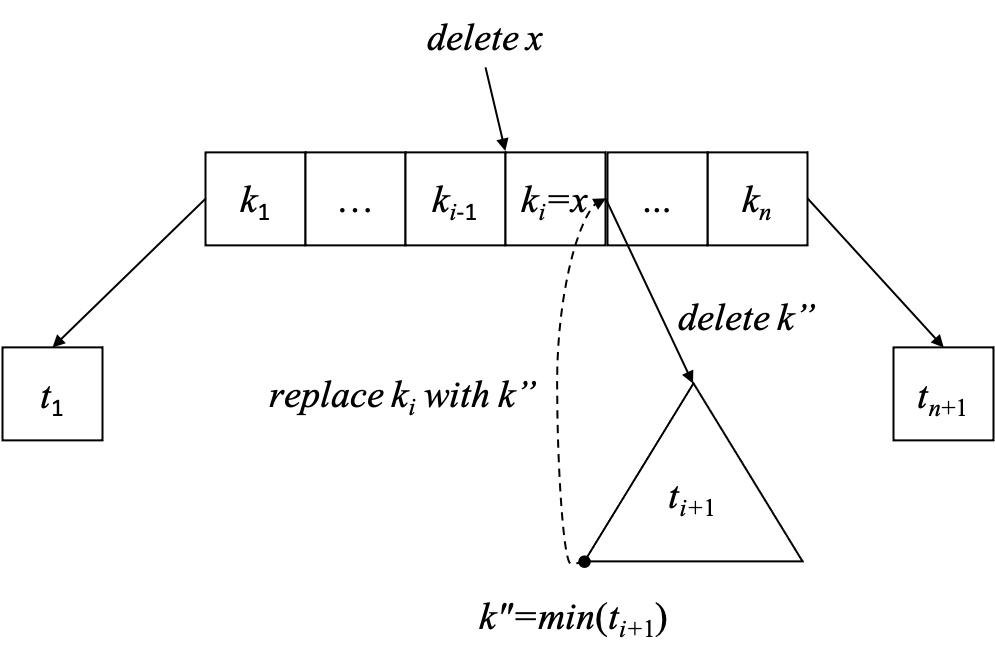
\includegraphics[scale=0.5]{img/btree-del-case2b.eps}
    \caption{使用后继元素替换并递归进行删除} \label{fig:btree-del-case2b}
\end{figure}

\item 子情况2c:否则,如果$y$和$z$含有的key都不足,我们可以将$y$、$k$和$z$合并成一个新节点,它恰好含有$2t-1$个key,此后,我们就可以针对这个新节点进行递归删除。

这里有一个特殊情况:如果合并后的节点不含有任何key,也就是说,$k$是$x$中的唯一key,而$y$和$z$是$x$仅有的两个子节点。这时我们需要将树的高度降低一层。
\end{itemize}

图\ref{fig:btree-del-case2c}描述了这种情况。

\begin{figure}[htbp]
  \centering
    \includegraphics[scale=0.5]{img/btree-del-case2c.eps}
    \caption{合并后再删除} \label{fig:btree-del-case2c}
\end{figure}

还有一种情况,如果$k$不是节点$x$中的key,我们需要在$x$中找到一个子节点$c_i$,使得$k$在子树$c_i$中。在对$c_i$进行递归删除前,我们需要预先确定$c_i$至少含有$t$个key。如果含有的key不足,就需要进行如下的调整。

\begin{itemize}
\item 子情况3a:我们检查$c_i$的前后兄弟节点$c_{i-1}$和$c_{i+1}$。如果任何一个节点包含有足够的key(至少$t$个),我们就将$x$中的一个key向下移动到$c_i$中,并将含有足够多key的兄弟节点中的一个key向上移动到$x$中。同时,我们还需要将兄弟节点中相应的子节点移动到$c_i$中。

这一操作使得$c_i$含有足够多的key以便进行后面的删除。接下来我们可以从$c_i$中递归删除$k$。

图\ref{fig:btree-del-case3a}描述了这一情况。

\begin{figure}[htbp]
  \centering
    \includegraphics[scale=0.5]{img/btree-del-case3a.eps}
    \caption{向右侧的兄弟节点“借”一个key}
    \label{fig:btree-del-case3a}
\end{figure}

\item 子情况3b:如果左右两个兄弟节点含有的key都不足,我们可以将$c_i$,$x$中的一个key,和任一兄弟节点合并为一个新节点。然后针对这一节点执行删除操作。
\end{itemize}

图\ref{fig:btree-del-case3b}描述了这一情况。

\begin{figure}[htbp]
  \centering
    \includegraphics[scale=0.5]{img/btree-del-case3b.eps}
    \caption{将$c_i$、$k$和$c_{i+1}$合并为一个新节点}
    \label{fig:btree-del-case3b}
\end{figure}

为了实现删除算法,我们需要先定义一些辅助函数。函数\textproc{Can-Del}检查一个节点是否含有足够多的key以执行删除操作。

\begin{algorithmic}[1]
\Function{Can-Del}{$T$}
  \State \Return $|K(T)| \ge t$
\EndFunction
\end{algorithmic}

过程\textproc{Merge-Children}($T, i$)将子节点$c_i(T)$、key $k_i(T)$和子节点$c_{i+1}(T)$合并成一个新节点。

\begin{algorithmic}[1]
\Procedure{Merge-Children}{$T, i$} \Comment{将$c_i(T)$、$k_i(T)$和$c_{i+1}(T)$合并}
  \State $x \gets c_i(T)$
  \State $y \gets c_{i+1}(T)$
  \State $K(x) \gets K(x) \cup \{k_i(T)\} \cup K(y)$
  \State $C(x) \gets C(x) \cup C(y)$
  \State \Call{Remove-At}{$K(T), i$}
  \State \Call{Remove-At}{$C(T), i+1$}
\EndProcedure
\end{algorithmic}

这一过程从给定的树$T$中定位到第$i$个子节点和key,将它们和第$i+1$个节点合并,然后从$T$中将第$i$个key和第$i+1$个子节点删除。

使用上述函数,我们可以分别处理三种不同的情况,从而定义下面的B树删除算法。

\begin{algorithmic}[1]
\Function{Delete}{$T, k$}
  \State $i \gets 1$
  \While{$i \leq |K(T)|$}
    \If{$k = k_i(T)$}
      \If{$T$ is leaf} \Comment{情况1}
        \State \Call{Remove}{$K(T), k$}
      \Else \Comment{情况2}
        \If{\Call{Can-Del}{$c_i(T)$}} \Comment{情况2a}
          \State $k_i(T) \gets$ \Call{Last-Key}{$c_i(T)$}
          \State \Call{Delete}{$c_i(T), k_i(T)$}
        \ElsIf{\Call{Can-Del}{$c_{i+1}(T)$}} \Comment{情况2b}
          \State $k_i(T) \gets$ \Call{First-Key}{$c_{i+1}(T)$}
          \State \Call{Delete}{$c_{i+1}(T), k_i(T)$}
        \Else \Comment{情况2c}
          \State \Call{Merge-Children}{$T, i$}
          \State \Call{Delete}{$c_i(T), k$}
          \If{$K(T) = NIL$}
            \State $T \gets c_i(T)$ \Comment{缩小高度}
          \EndIf
        \EndIf
      \EndIf
      \State \Return $T$
    \ElsIf{$k < k_i(T)$}
      \State Break
    \Else
      \State $i \gets i+1$
    \EndIf
  \EndWhile
  \Statex
  \If{$T$ is leaf}
    \State \Return $T$ \Comment{$k$不在$T$中}
  \EndIf
  \If{$\lnot$ \Call{Can-Del}{$c_i(T)$}}  \Comment{情况3}
    \If{$i>1 \land$ \Call{Can-Del}{$c_{i-1}(T)$}} \Comment{情况3a:左侧兄弟}
      \State \Call{Insert}{$K(c_i(T)), k_{i-1}(T)$}
      \State $k_{i-1}(T) \gets$ \Call{Pop-Back}{$K(c_{i-1}(T))$}
      \If{$c_i(T)$ isn't leaf}
        \State $c \gets$ \Call{Pop-Back}{$C(c_{i-1}(T))$}
        \State \Call{Insert}{$C(c_i(T)), c$}
      \EndIf
    \ElsIf{$i \leq |C(T)| \land$ \Call{Can-Del}{$c_{i_1}(T)$}} \Comment{情况3a:右侧兄弟}
      \State \Call{Append}{$K(c_i(T)), k_i(T)$}
      \State $k_i(T) \gets$ \Call{Pop-Front}{$K(c_{i+1}(T))$}
      \If{$c_i(T)$ isn't leaf}
        \State $c \gets$ \Call{Pop-Front}{$C(c_{i+1}(T))$}
        \State \Call{Append}{$C(c_i(T)), c$}
      \EndIf
    \Else \Comment{情况3b}
      \If{$i>1$}
        \State \Call{Merge-Children}{$T, i-1$}
      \Else
        \State \Call{Merge-Children}{$T, i$}
      \EndIf
    \EndIf
  \EndIf
  \State \Call{Delete}{$c_i(T), k$} \Comment {递归删除}
  \If{$K(T) = NIL$} \Comment {缩小高度}
    \State $T \gets c_1(T)$
  \EndIf
  \State \Return $T$
\EndFunction
\end{algorithmic}

图\ref{fig:result-del1}、\ref{fig:result-del2}和\ref{fig:result-del3}描述了删除中的各个步骤,被改变的节点用灰色显示。

\begin{figure}[htbp]
  \centering
  \subcaptionbox{删除前的B树}{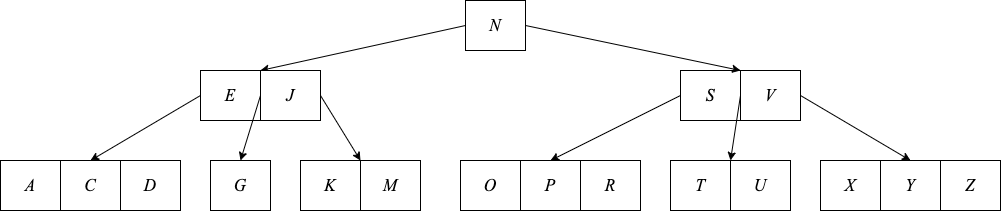
\includegraphics[scale=0.5]{img/btree-del-before.ps}} \\
  \subcaptionbox{删除key ‘F’,情况1}{\includegraphics[scale=0.5]{img/btree-del-F.ps}}
  \caption{B树删除的结果(1)} \label{fig:result-del1}
\end{figure}

\begin{figure}[htbp]
  \centering
  \subcaptionbox{删除key ‘M’后,子情况2a}{\includegraphics[scale=0.5]{img/btree-del-M.ps}} \\
  \subcaptionbox{删除key ‘G’后,子情况2c}{\includegraphics[scale=0.5]{img/btree-del-G.ps}}
  \caption{B树删除的结果(2)} \label{fig:result-del2}
\end{figure}

\begin{figure}[htbp]
  \centering
  \subcaptionbox{删除key ‘D’后,子情况3b,树的高度减少1}{\includegraphics[scale=0.5]{img/btree-del-D.ps}} \\
  \subcaptionbox{删除key ‘B’后,子情况3a,向右侧兄弟节点”借“一个key}{\includegraphics[scale=0.5]{img/btree-del-B.ps}} \\
  \subcaptionbox{删除key ‘U’后,子情况3a,向左侧兄弟节点“借”一个key}{\includegraphics[scale=0.5]{img/btree-del-U.ps}}
  \caption{B树删除的结果(3)} \label{fig:result-del3}
\end{figure}

下面的Python例子程序实现了B树的删除算法。

\lstset{language=Python}
\begin{lstlisting}
def can_remove(tr):
    return len(tr.keys) >= tr.t

def replace_key(tr, i, k):
    tr.keys[i] = k
    return k

def merge_children(tr, i):
    tr.children[i].keys += [tr.keys[i]] + tr.children[i+1].keys
    tr.children[i].children += tr.children[i+1].children
    tr.keys.pop(i)
    tr.children.pop(i+1)

def B_tree_delete(tr, key):
    i = len(tr.keys)
    while i>0:
        if key == tr.keys[i-1]:
            if tr.leaf:  # 情况1
                tr.keys.remove(key)
            else: # 情况2
                if tr.children[i-1].can_remove(): # 情况2a
                    key = tr.replace_key(i-1, tr.children[i-1].keys[-1])
                    B_tree_delete(tr.children[i-1], key)
                elif tr.children[i].can_remove(): # 情况2b
                    key = tr.replace_key(i-1, tr.children[i].keys[0])
                    B_tree_delete(tr.children[i], key)
                else: # 情况2c
                    tr.merge_children(i-1)
                    B_tree_delete(tr.children[i-1], key)
                    if tr.keys==[]: # 缩减树的高度
                        tr = tr.children[i-1]
            return tr
        elif key > tr.keys[i-1]:
            break
        else:
            i = i-1
    # 情况3
    if tr.leaf:
        return tr # key不存在
    if not tr.children[i].can_remove():
        # 情况3a
        if i>0 and tr.children[i-1].can_remove(): # 左侧兄弟
            tr.children[i].keys.insert(0, tr.keys[i-1])
            tr.keys[i-1] = tr.children[i-1].keys.pop()
            if not tr.children[i].leaf:
                tr.children[i].children.insert(0, tr.children[i-1].children.pop())
        elif i<len(tr.children) and tr.children[i+1].can_remove(): # 右侧兄弟
            tr.children[i].keys.append(tr.keys[i])
            tr.keys[i]=tr.children[i+1].keys.pop(0)
            if not tr.children[i].leaf:
                tr.children[i].children.append(tr.children[i+1].children.pop(0))
        else: # 情况3b
            if i>0:
                tr.merge_children(i-1)
            else:
                tr.merge_children(i)
    B_tree_delete(tr.children[i], key)
    if tr.keys==[]: # 缩减树的高度
        tr = tr.children[0]
    return tr
\end{lstlisting}

% ================================================================
%               Delete and fix method
% ================================================================

\subsection{先删除再修复}

删除前预合并算法比较复杂了,需要处理不同的情况,每种情况又含有若干子情况。

我们也可以换一种思路来设计删除算法。即先删除,然后再进行必要的修复。这种策略和先插入再修复相类似。

\be
delete(T, k) = fix(del(T, k))
\ee

从B树删除一个key时,我们先从根节点开始,自顶向下定位到这个key所在的节点。

如果这一节点是一个叶子节点,我们就删掉相应的key,然后检查节点种剩余的key是否太少以至于无法满足B树的平衡条件。

如果这一节点是一个分支节点,删掉key后它就被分为两部分。我们合并它们。这一合并过程是递归的,如图\ref{fig:del-fp-merge}所示。

\begin{figure}[htbp]
  \centering
  \includegraphics[scale=0.5]{img/btree-del-fp-merge.eps}
  \caption{从分支节点种删除key。删除$k_i$后节点分成了两部分。递归将它们合并直到这两部分都是叶子节点。} \label{fig:del-fp-merge}
\end{figure}

合并时,如果待合并的两个节点不是叶子节点,我们将key合到一起,然后递归地将左侧部分的最后一个子树和右侧部分的第一个子树合并。否则,如果它们都是叶子节点,我们只需要将key合并到一起。

到目前为止,待删除的key已经从树中去掉了。但是由此导致节点中key的减少可能会违反B树的平衡条件。我们需要从根节点开始,沿着删除时经过的路径进行修复。

\begin{figure}[htbp]
  \centering
  \includegraphics[scale=0.5]{img/btree-del-fp-make.eps}
  \caption{从节点$c_i$中删除key $k$后,结果为$c_i'$。修复时,我们用左侧部分、$c_i'$和右侧部分构造一个新节点。}
  \label{fig:del-fp-make}
\end{figure}

经过递归删除,路径上的任何一个分支节点都被分成了三部分:左侧部分包含了所有不大于$k$的key,包括$k_1, k_2, ..., k_{i-1}$和子树$c_1, c_2, ..., c_{i-1}$;右侧部分包含了全部不小于$k$的key,包括$k_i, k_{i+1}, ..., k_{n+1}$和子树$c_{i+1}, c_{i+2}, ..., c_{n+1}$;$k$被递归地从子树$c_i$中删除,我们将结果记为$c_i'$。如图\ref{fig:del-fp-make}所示。

此时,我们需要检查$c_i'$是否包含了足够多的key。如果不足(少于$t-1$个,注意这里和删除前预合并不同,后者判断是否少于$t$个),我们可以从左侧,或者右侧“借”来一对key和子树,这是分拆操作的逆向操作。图\ref{fig:del-fp-fixlow}描述了向左侧“借”一对key和子树的情形。

\begin{figure}[htbp]
  \centering
  \includegraphics[scale=0.5]{img/btree-del-fp-fixlow.eps}
  \caption{向左侧部分“借”一对key和子树,然后进行分拆的逆操作} \label{fig:del-fp-fixlow}
\end{figure}

如果左侧和右侧都为空,我们只需要把$c_i'$推向上层。

记B树为$T=(K, C, t)$,其中$K$和$C$分别为key和子树。函数$del(T, k$)从树中删除key $k$。

\be
del(T, k) = \left \{
  \begin{array}
  {r@{\quad:\quad}l}
  (delete(K, k), \phi, t) & C = \phi \\
  merge((K_1, C_1, t), (K_2, C_2, t)) & k_i = k \\
  make((K_1', C_1'), del(c, k), (K_2', C_2')) & k \notin K
  \end{array}
\right.
\ee

如果没有任何子树$C = \phi$,说明$T$是一叶子节点。我们直接将$k$删除。否则,$T$为一个内部分支节点。如果$k \in K$,将$k$删除后所有的key和子树被分成了两部分:$(K_1, C_1)$和$(K_2, C_2)$。它们接下来被递归地合并。

\[
\begin{array}{l}
K_1 = \{k_1, k_2, ..., k_{i-1}\} \\
K_2 = \{k_{i+1}, k_{i+2}, ..., k_m\} \\
C_1 = \{c_1, c_2, ..., c_i\} \\
C_2 = \{c_{i+1}, c_{i+2}, ..., c_{m+1}\}
\end{array}
\]

如果$k \notin K$,我们需要定位到一个子树$c$,然后递归地从这个子树中删除$k$。

\[
\begin{array}{l}
(K_1', K_2') = (\{k' | k' \in K, k' < k \}, \{k' | k' \in K, k < k' \}) \\
(C_1', \{c\} \cup C_2') = splitAt(|K_1'|, C)
\end{array}
\]

递归合并函数被定义如下:当合并两棵树$T_1 = (K_1, C_1, t)$和$T_2 = (K_2, C_2, t)$时,如果它们都是叶子节点,我们将两组key连接到一起形成一个新的叶子节点。否则,我们将$C_1$中的最后一棵子树和$C_2$中的第一棵子树递归合并。然后调用$make$函数构造一棵新树。若$C_1$和$C_2$不为空,记$C_1$中的最后一棵子树为$c_{1, m}$,其余子树为$C_1'$;记$C_2$中的第一棵子树为$C_{2, 1}$,其余子树为$C_2'$。下面的公式定义了合并函数:

\be
merge(T_1, T_2) = \left \{
  \begin{array}
  {r@{\quad:\quad}l}
  (K_1 \cup K_2, \phi, t) & C_1 = C_2 = \phi \\
  make((K_1, C_1'), merge(c_{1,m}, c_{2, 1}), (K_2, C_2')) & otherwise
  \end{array}
\right.
\ee

我们此前定义的$make$函数仅仅处理了由于插入造成节点中含有过多key的情况。我们可以对它进行修改,使得它能够处理由于删除造成key过少的情况。

\be
make((K', C'), c, (K'', C'')) = \left \{
  \begin{array}
  {r@{\quad:\quad}l}
  fixFull((K', C'), c, (K'', C'')) & full(c) \\
  fixLow((K', C'), c, (K'', C'')) & low(c) \\
  (K' \cup K'', C' \cup \{c\} \cup C'', t) & otherwise
  \end{array}
\right.
\ee

其中$low(T)$检查节点$T$含有的key是否少于$t-1$。函数$fixLow(P_l, c, P_r)$接受三个参数:左侧的key和子树对$P_l$、一个子节点$c$、以及右侧的key和子树对$P_r$。如果左侧部分不为空,我们就从左侧“借”一对key和子树,然后进行逆分拆操作使得节点含有足够多的key,然后递归地调用$make$。否则,如果右侧不为空,我们就向右侧“借”一对key和子树。如果左右都为空,我们就将子节点直接返回作为结果。这种情况下,树的高度会减低。

令左侧部分为$P_l = (K_l, C_l)$,如果$K_l$不为空,记最后一对key和子树分别为$k_{l, m}$和$c_{l, m}$。剩余的key和子树记为$K_l'$ and $C_l'$。同样,令右侧部分为$P_r = (K_r, C_r)$,如果$K_r$不为空,记第一对key和子树分别为$k_{r, 1}$和$c_{r, 1}$。剩余的key和子树记为$K_r'$ and $C_r'$。函数$fixLow$定义如下:

\be
fixLow(P_l, c, P_r) = \left \{
  \begin{array}
  {r@{\quad:\quad}l}
  make((K_l', C_l'), unsplit(c_{l, m}, k_{l, m}, c), (K_r, C_r)) & K_l \neq \phi \\
  make((K_r, C_r), unsplit(c, k_{r, 1}, c_{r, 1}), (K_r', C_r')) & K_r \neq \phi \\
  c & otherwise
  \end{array}
\right.
\ee

函数$unsplit(T_1, k, T_2)$是分拆的逆操作,它用两个子树和一个key构造一棵新的B树。

\be
unsplit(T_1, k, T_2) = (K_1 \cup \{k\} \cup K_2, C_1 \cup C_2, t)
\ee

下面的Haskell例子程序实现了B树的删除算法。

\lstset{language=Haskell}
\begin{lstlisting}[style=Haskell]
import qualified Data.List as L

delete tr x = fixRoot $ del tr x

del:: (Ord a) => BTree a -> a -> BTree a
del (Node ks [] t) x = Node (L.delete x ks) [] t
del (Node ks cs t) x =
    case L.elemIndex x ks of
      Just i -> merge (Node (take i ks) (take (i+1) cs) t)
                      (Node (drop (i+1) ks) (drop (i+1) cs) t)
      Nothing -> make (ks', cs') (del c x) (ks'', cs'')
    where
      (ks', ks'') = L.partition (<x) ks
      (cs', (c:cs'')) = L.splitAt (length ks') cs

merge (Node ks [] t) (Node ks' [] _) = Node (ks++ks') [] t
merge (Node ks cs t) (Node ks' cs' _) = make (ks, init cs)
                                             (merge (last cs) (head cs'))
                                             (ks', tail cs')

make (ks', cs') c (ks'', cs'')
    | full c = fixFull (ks', cs') c (ks'', cs'')
    | low c  = fixLow  (ks', cs') c (ks'', cs'')
    | otherwise = Node (ks'++ks'') (cs'++[c]++cs'') (degree c)

low tr = (length $ keys tr) < (degree tr)-1

fixLow (ks'@(_:_), cs') c (ks'', cs'') = make (init ks', init cs')
                                              (unsplit (last cs') (last ks') c)
                                              (ks'', cs'')
fixLow (ks', cs') c (ks''@(_:_), cs'') = make (ks', cs')
                                              (unsplit c (head ks'') (head cs''))
                                              (tail ks'', tail cs'')
fixLow _ c _ = c

unsplit c1 k c2 = Node ((keys c1)++[k]++(keys c2))
                       ((children c1)++(children c2)) (degree c1)
\end{lstlisting}

使用先删除再修复的方法从同样的B树中依次删除同样的key,得到的结果和删除前预合并的有所不同,如图\ref{fig:result-del-fp1}、\ref{fig:result-del-fp2}和\ref{fig:result-del-fp3}。但是它们都是满足平衡条件的合法的B树。

\begin{figure}[htbp]
  \centering
  \subcaptionbox{删除前的B树}{\includegraphics[scale=0.5]{img/btree-del-fp-before.ps}}\\
  \subcaptionbox{删除key ‘E’后}{\includegraphics[scale=0.5]{img/btree-del-fp-E.ps}}
  \caption{先删除再修复的结果(1)} \label{fig:result-del-fp1}
\end{figure}

\begin{figure}[htbp]
  \centering
  \subcaptionbox{删除key ‘G’后}{\includegraphics[scale=0.5]{img/btree-del-fp-G.ps}} \\
  \subcaptionbox{删除key ‘A’后}{\includegraphics[scale=0.5]{img/btree-del-fp-A.ps}}
  \caption{先删除再修复的结果(2)} \label{fig:result-del-fp2}
\end{figure}

\begin{figure}[htbp]
  \centering
  \subcaptionbox{删除key ‘M’后}{\includegraphics[scale=0.5]{img/btree-del-fp-M.ps}} \\
  \subcaptionbox{删除key ‘U’后}{\includegraphics[scale=0.5]{img/btree-del-fp-U.ps}}
  \caption{先删除再修复的结果(3)} \label{fig:result-del-fp3}
\end{figure}


% ================================================================
%               Searching
% ================================================================
\section{搜索}
\index{B树!搜索}

我们可以将二叉搜索树的搜索算法进行抽象概括,从而获得B树的搜索算法。

对于二叉树,每次只有两种选择,或者向左,或者向右。但是B树中存在多个选择。

\begin{algorithmic}[1]
\Function{Search}{$T, k$}
  \Loop
    \State $i \gets 1$
    \While{$i \leq |K(T)| \land k > k_i(T)$}
      \State $i \gets i+1$
    \EndWhile
    \If{$i \leq |K(T)| \land k = k_i(T)$}
      \State \Return $(T, i)$
    \EndIf
    \If{$T$ is leaf}
      \State \Return $NIL$ \Comment{$k$不存在}
    \Else
      \State $T \gets c_i(T)$
    \EndIf
  \EndLoop
\EndFunction
\end{algorithmic}

从根节点开始,算法按照从小到大的顺序逐一检查每个key。如果发现匹配的key,就返回当前节点和key的索引作为结果。否则,如果找到某一位置$i$使得$k_i < k < k_{i+1}$,接下来就在子树$c_{i+1}$中搜索这一key。如果到达了某一叶子节点还没有找到key,就返回一个空值表示不存在。

下面的Python例子程序实现了B树搜索算法。

\lstset{language=Python}
\begin{lstlisting}
def B_tree_search(tr, key):
    while True:
        for i in range(len(tr.keys)):
            if key <= tr.keys[i]:
                break
        if key == tr.keys[i]:
            return (tr, i)
        if tr.leaf:
            return None
        else:
            if key > tr.keys[-1]:
                i=i+1
            tr = tr.children[i]
\end{lstlisting}

也可以用递归的方式实现B树搜索算法。当在B树$T = (K, C, t)$中搜索key $k$时,我们首先使用$k$将所有的key分成两部分。

\[
\begin{array}{l}
K_1 = \{ k' | k' < k \} \\
K_2 = \{ k' | k \leq k' \}
\end{array}
\]

即$K_1$包含所有小于$k$的key;而$K_2$包含其余的部分。如果$K_2$的第一个元素恰好等于$k$,则搜索成功,否则我们需要递归地在子树$c_{|K_1|+1}$中搜索。

\be
search(T, k) = \left \{
  \begin{array}
  {r@{\quad:\quad}l}
  (T, |K_1|+1) & k \in K_2 \\
  \phi & C = \phi \\
  search(c_{|K_1|+1}, k) & otherwise
  \end{array}
\right.
\ee

下面的Haskell例子程序实现了这一算法。

\lstset{language=Haskell}
\begin{lstlisting}[style=Haskell]
search :: (Ord a)=> BTree a -> a -> Maybe (BTree a, Int)
search tr@(Node ks cs _) k
    | matchFirst k $ drop len ks = Just (tr, len)
    | otherwise = if null cs then Nothing
                  else search (cs !! len) k
    where
      matchFirst x (y:_) = x==y
      matchFirst x _ = False
      len = length $ filter (<k) ks
\end{lstlisting}


% ================================================================
%                 Short summary
% ================================================================
\section{小结}

本章中,我们介绍了B树,它是二叉搜索树的一种扩展。我们跳过了有关磁盘访问的背景知识,读者可以参考\cite{CLRS}加以了解。我们给出了主要三种操作:插入、删除和查找的命令式和函数式算法。它们都从根节点向叶子节点进行查找,算法执行的时间和树的高度成正比。由于B树总是平衡的,因此对于含有$n$个元素的B树,这些操作的时间就可以保证是$O(\lg n)$的。

\begin{Exercise}
\begin{itemize}
\item 在插入时,我们需要找到合适的位置,使得左侧的key都小于待插入的元素,而右侧的key都大于它。实际上,元素只要支持小于和等于比较就可以了。请改动插入算法,放松这一限制。
\item 我们假设B树中不存在待插入的元素。修改算法使得重复的元素保存在一链表中。
\item 修改命令式B树算法,去除其中的递归调用。
\end{itemize}
\end{Exercise}

\ifx\wholebook\relax \else
\begin{thebibliography}{99}

\bibitem{CLRS}
Thomas H. Cormen, Charles E. Leiserson, Ronald L. Rivest and Clifford Stein. ``Introduction to Algorithms, Second Edition''. The MIT Press, 2001. ISBN: 0262032937.(《算法导论》第二版)

\bibitem{wiki-b-tree}
B-tree, Wikipedia. http://en.wikipedia.org/wiki/B-tree

\bibitem{okasaki}
Chris Okasaki. ``FUNCTIONAL PEARLS Red-Black Trees in a Functional Setting''. J. Functional Programming. 1998

\end{thebibliography}

\end{document}
\fi
